\documentclass[11pt,a4paper]{letter}
\usepackage[top=1.00in, bottom=1.0in, left=.75in, right=0.75in]{geometry}
\usepackage{graphicx}
\usepackage{natbib}

\address{1300 Centre Street \\ Boston, MA, 20131}

\begin{document}
\bibliographystyle{..//..//refs/bibstyles/amnat.bst}
\begin{letter}{}
\includegraphics[width=0.5\textwidth]{/Users/aileneettinger/Dropbox/Documents/Work/AA_heading.pdf}
\pagenumbering{gobble}

\opening{Dear Dr. Findlay:}
We propose a ``Perspective" on implications of the altered photoperiod that many organisms will experience as they shift their ranges or seasonal activities with climate change. 
We believe this piece would be of broad interest to readers of \emph{Nature Climate Change}, as altered photoperiod could have wide-reaching impacts on most plant and animal species. Photoperiod acts as a cue for the spring emergence and migration timing of diverse species, and alterations to experienced photoperiod can therefore affect development, growth, and fitness for plants, insects, fish, and mammals, among other organisms. Thus, understanding and forecasting these changes is critical for biologists forecasting species responses, policy-makers dependent on these forecasts for adaptation strategies and all those dependent on the services provided by these species. Yet, photoperiod has rarely been included in forecasts of responses to climate change and implications of climate change induced shifts in photoperiod are largely unexplored, especially for early-season spring events, where changes will be most dramatic. 
\\
\\
The two most observed impacts of climate change on species are shifts in space (altitudinal and latitudinal range shifts) and in time (phenological shifts) (Chen et al 2011, Parmesan and Yohe 2003) and both result in altered photoperiod regimes (Saikkonen et al 2012).  Altered photoperiods have the potential to dramatically alter species' performance and fitness, however, the magnitude of effects of shifts in photoperiod with climate change are unknown or unquantified for the vast majority of species.  Our Perspective would quantify expected changes in experienced photoperiod due to shifts in space versus in time, given observations to date (e.g., Chen et al 2011, Parmesan and Yohe 2003), and put them in a novel, global context. Previous work has focused on effects geographic shifts in species distributions on photoperiod (e,g,, Saikkonen et al 2012, Way and Montgomery 2015), yet we will demonstrate that impacts on experienced photoperiod due to temporal shifts may be orders of magnitude larger than impacts due to spatial shifts (e.g., 1.6 hours of change versus one minute of change, Figure 1). 
\\
\\
Our Perspective would also offer a valuable addition to current approaches because it would focus on spring phenology events. To date, the role of photoperiod has received far more detailed attention for end-of-season activities, such as growth cessation in the fall than for spring. Though photoperiod cues dominate in the fall for many organisms, fall phenology responses to climate change have been muted. In contrast, spring phenology responds strongly to temperature and thus has advanced substantially with warming---causing cascading, and generally unexplored, effects on photoperiod experienced at the start of spring. With continued warming photoperiod limitations could come into play, however, and cause the rapidly advancing springs to abruptly slow or stall. We will demonstrate that incorporating photoperiod into forecasts is possible by leveraging existing experimental data (cite ospree XX database). For example, growth chamber experiments on woody plant spring phenology often have data relevant for climate change impacts. We plan to highlight how new modelling approaches can improve predictions of when, where, and how much photoperiod is likely to affect future spring phenology and could be combined with new empirical work to advance our understanding of the role of photoperiod in a warming world.%Figure of conceptual diagram 
\\
\\
We expect the title of our manuscript to be ``Spatial and temporal shifts in photoperiod with climate change."  It will be co-authored by D. Buonaiuto, C. Chamberlain, I. Morales-Castilla, and E. Wolkovich. Thank you for considering our paper.

Sincerely,\\

\includegraphics[scale=1]{/Users/aileneettinger/Dropbox/Documents/Work/AileneEttingerSignature.png} \\
Ailene Ettinger, on behalf of all authors.
NRC Research Assocaite, Northwest Fisheries Science Center

\noindent \emph{References mentioned in cover letter}
\begin{footnotesize}
\begin{enumerate}
\item Chen, I.-C., J. K. Hill, R. Ohlemueller, D. B. Roy, and C. D. Thomas. 2011. Rapid range shifts of species associated with high levels of climate warming.  \emph{Science} 333:1024-1026.

\item Parmesan, C. and Yohe, G., 2003. A globally coherent fingerprint of climate change impacts across natural systems.  \emph{Nature}, 421:37.

\item Parmesan, C., 2006. Ecological and evolutionary responses to recent climate change.  \emph{Annu. Rev. Ecol. Evol. Syst.}, 37: 637-669.

\item Saikkonen, K., K. Taulavuori, T. Hyvonen, P. E. Gundel, C. E. Hamilton, I. Vanninen, A. Nissinen, and M. Helander. 2012. Climate change-driven species' range shifts filtered by photoperiodism. \emph{Nature Climate Change} 2:239.

\item Way, D. A., and R. A. Montgomery. 2015. Photoperiod constraints on tree phenology, performance and migration in a warming world. \emph{Plant, Cell \& Environment} 38:1725-1736.

\end{enumerate}
\end{footnotesize}

\begin{figure}

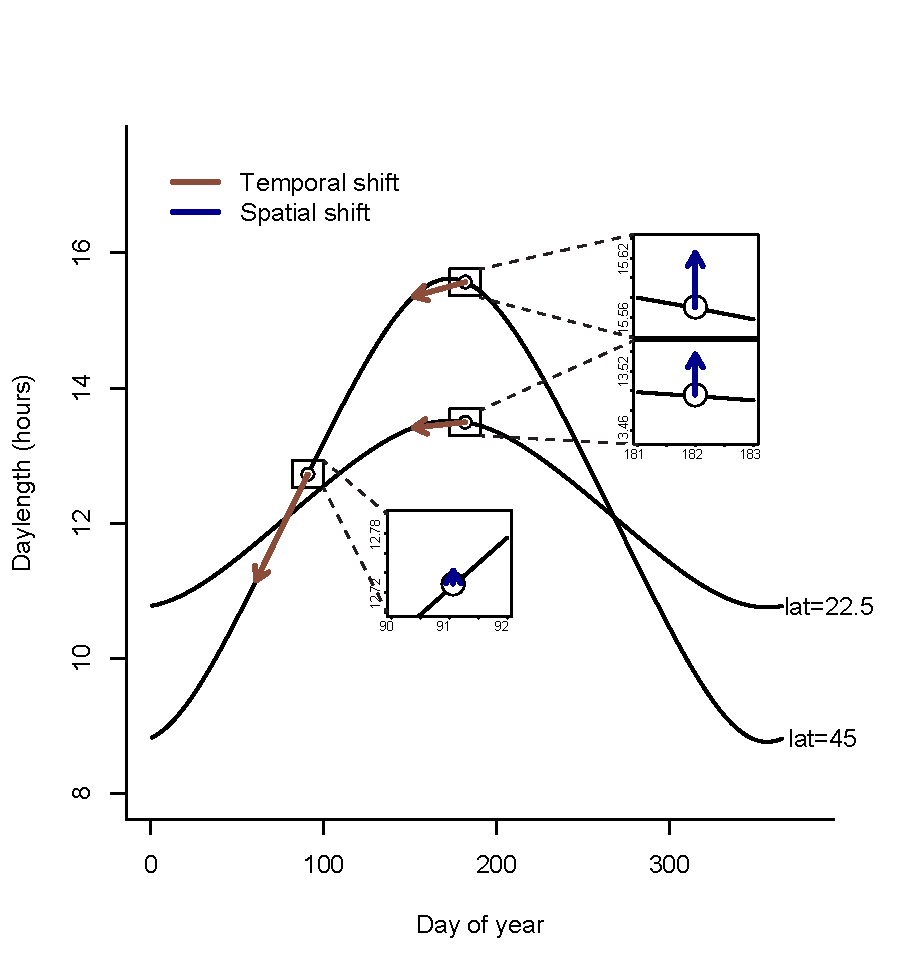
\includegraphics[width=180mm,scale=0.5]{..//..//analyses/photoperiod/figures/photo_spacetime_v2.pdf} 
\caption{\textbf{Figure 1: Photoperiod varies with latitude and by day of year, such that temporal shifts in
activity yield larger changes in experienced photoperiod compared with spatial shifts. Here, we show
this variation at two latitudes (22.5\degree, 45\degree), using hypothetical spatial and temporal shifts. These shifts,
which are similar to observed average rates with recent global warming (e.g., Parmesan, 2006; Chen
et al., 2011), highlight the greater magnitude in daylength changes close to the equinox (e.g., day of
year 91), versus close to the summer solstice (e.g., day of year 182).}
 \label{fig:condiag}
 \end{figure}

\end{letter}
\end{document}
